\section{Data Collection}
\label{data_collection}

In order to start working, we obviously needed some data. This section presents the three methods we used in order to get samples of acceleration data. The resulting datasets will be analysed (Section \ref{data_analysis}) and tested in order to find the best way to collect such data on a vehicle.

\subsection{Robot}
Being able to collect our own data is a huge advantage because we can also record metadata that can become handy for better understanding the raw accelerometric data but also for future experiments (for instance, comparing two captors or their placement on the vehicle).\\

It was possible thanks to the acquisition of a brand new radio-controled robot for the Télécom Physique Strasbourg Innov'Lab. This vehicle robot, an Agile-X Scout 2.0, is built for outdoor operations meaning it is perfectly suited to roll on bumps and cracks we had already spotted in the school parking lot.\\

Instead of waiting for our application, we decided to speed-up the process by using an Arduino to collect data. We paired an Arduino Nano with a fairly affordable but reliable IMU: an MPU-6050, which is a common module for DIY drones hobbyists and a micro-SD card module in order to record acceleration data. At the beginning, we also wanted to connect a \textit{Real Time Clock} (RTC) module and a GPS module (respectively a DS1307 and a BN-880) in order to track both time and position but we had to settle back for only acceleration data due to Arduino and I²C bus limitations.\\

After a lot of prototyping and debugging (Figure \ref{bread}), we were finally ready to build a \textit{Printed Circuit Board} (PCB) to conveniently hold the components together, removing any risk of disconnection during data collection. We designed the PCB with Ki-Cad (Figure \ref{pcb_preview}) and quickly made two of them with the school FabLab milling machine (Figure \ref{}).\\

In order to properly mount this little device on the robot, we designed a mounting plate in Solidworks that would acomodate us with many mounting holes for both attaching the plate on the robot and securing our devices on the plate. A FabLab manager helped us to laser-cut it in a large piece of acrylic (Figure \ref{robot_1}).\\

\begin{figure}
    \center
    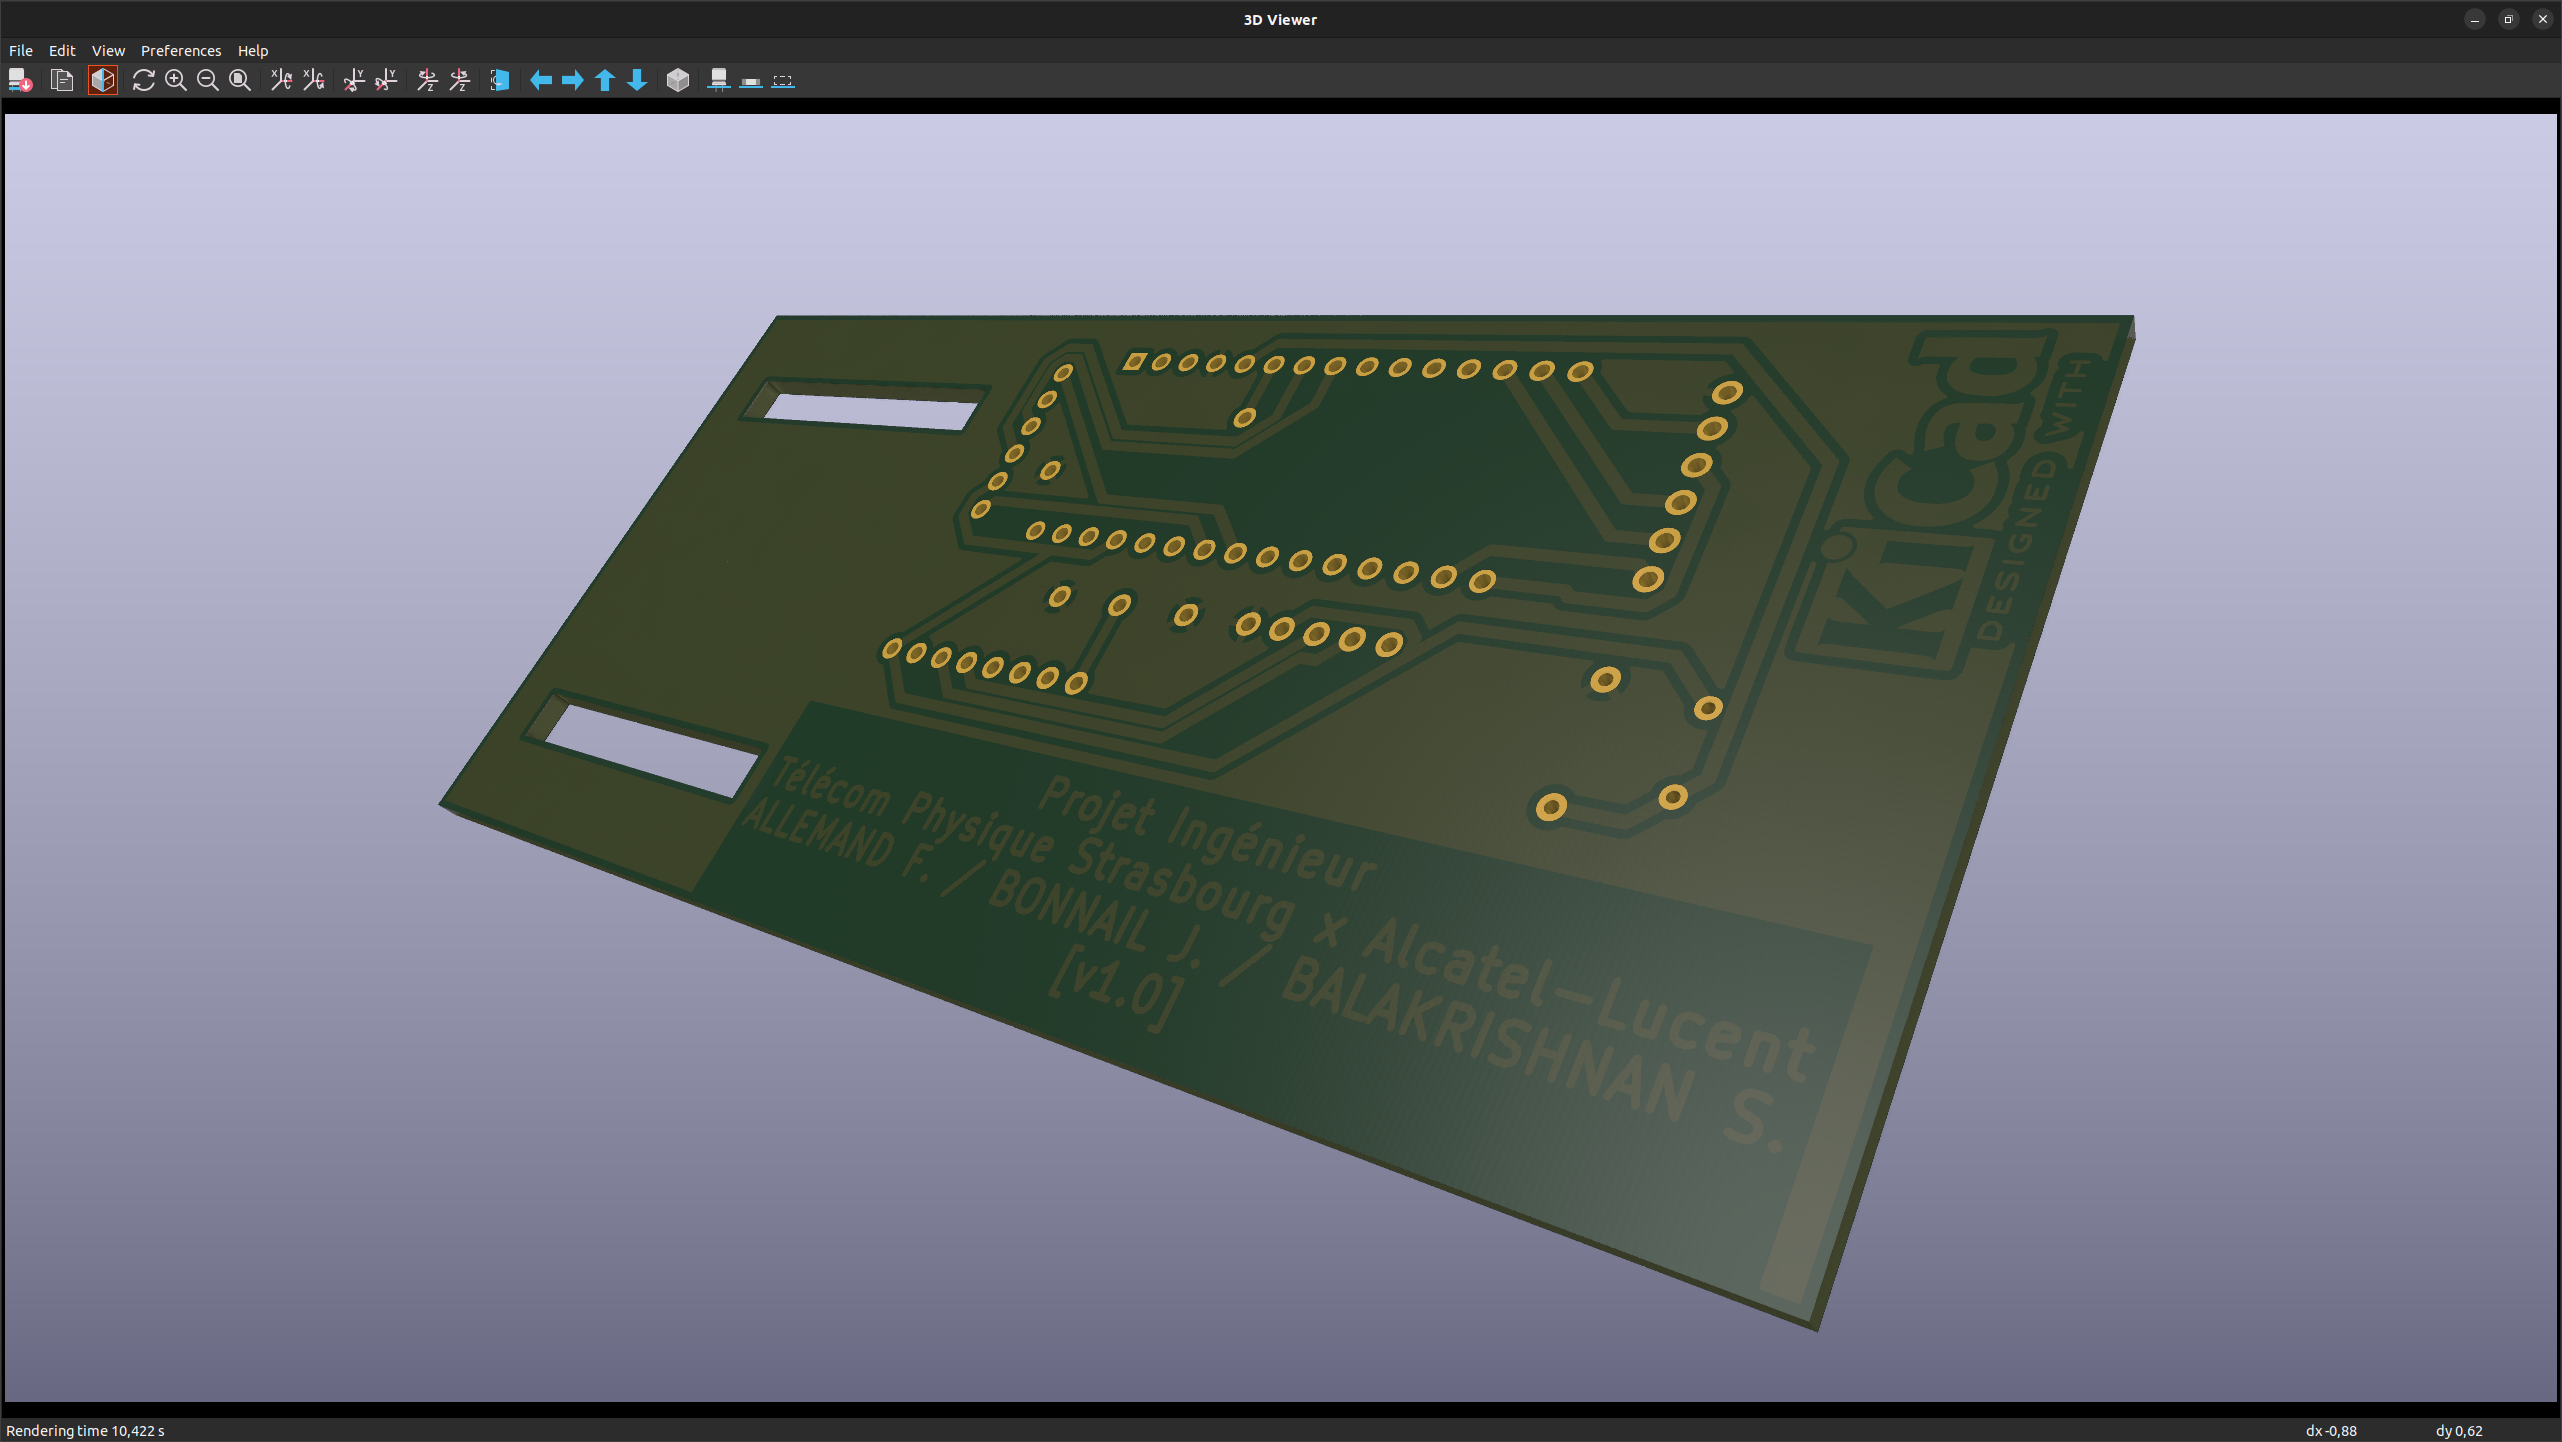
\includegraphics[scale=.12]{img/pcb_preview.png}
    \caption{Preview of the Arduino device PCB}
    \label{pcb_preview}
\end{figure}

\begin{figure}
    \center
    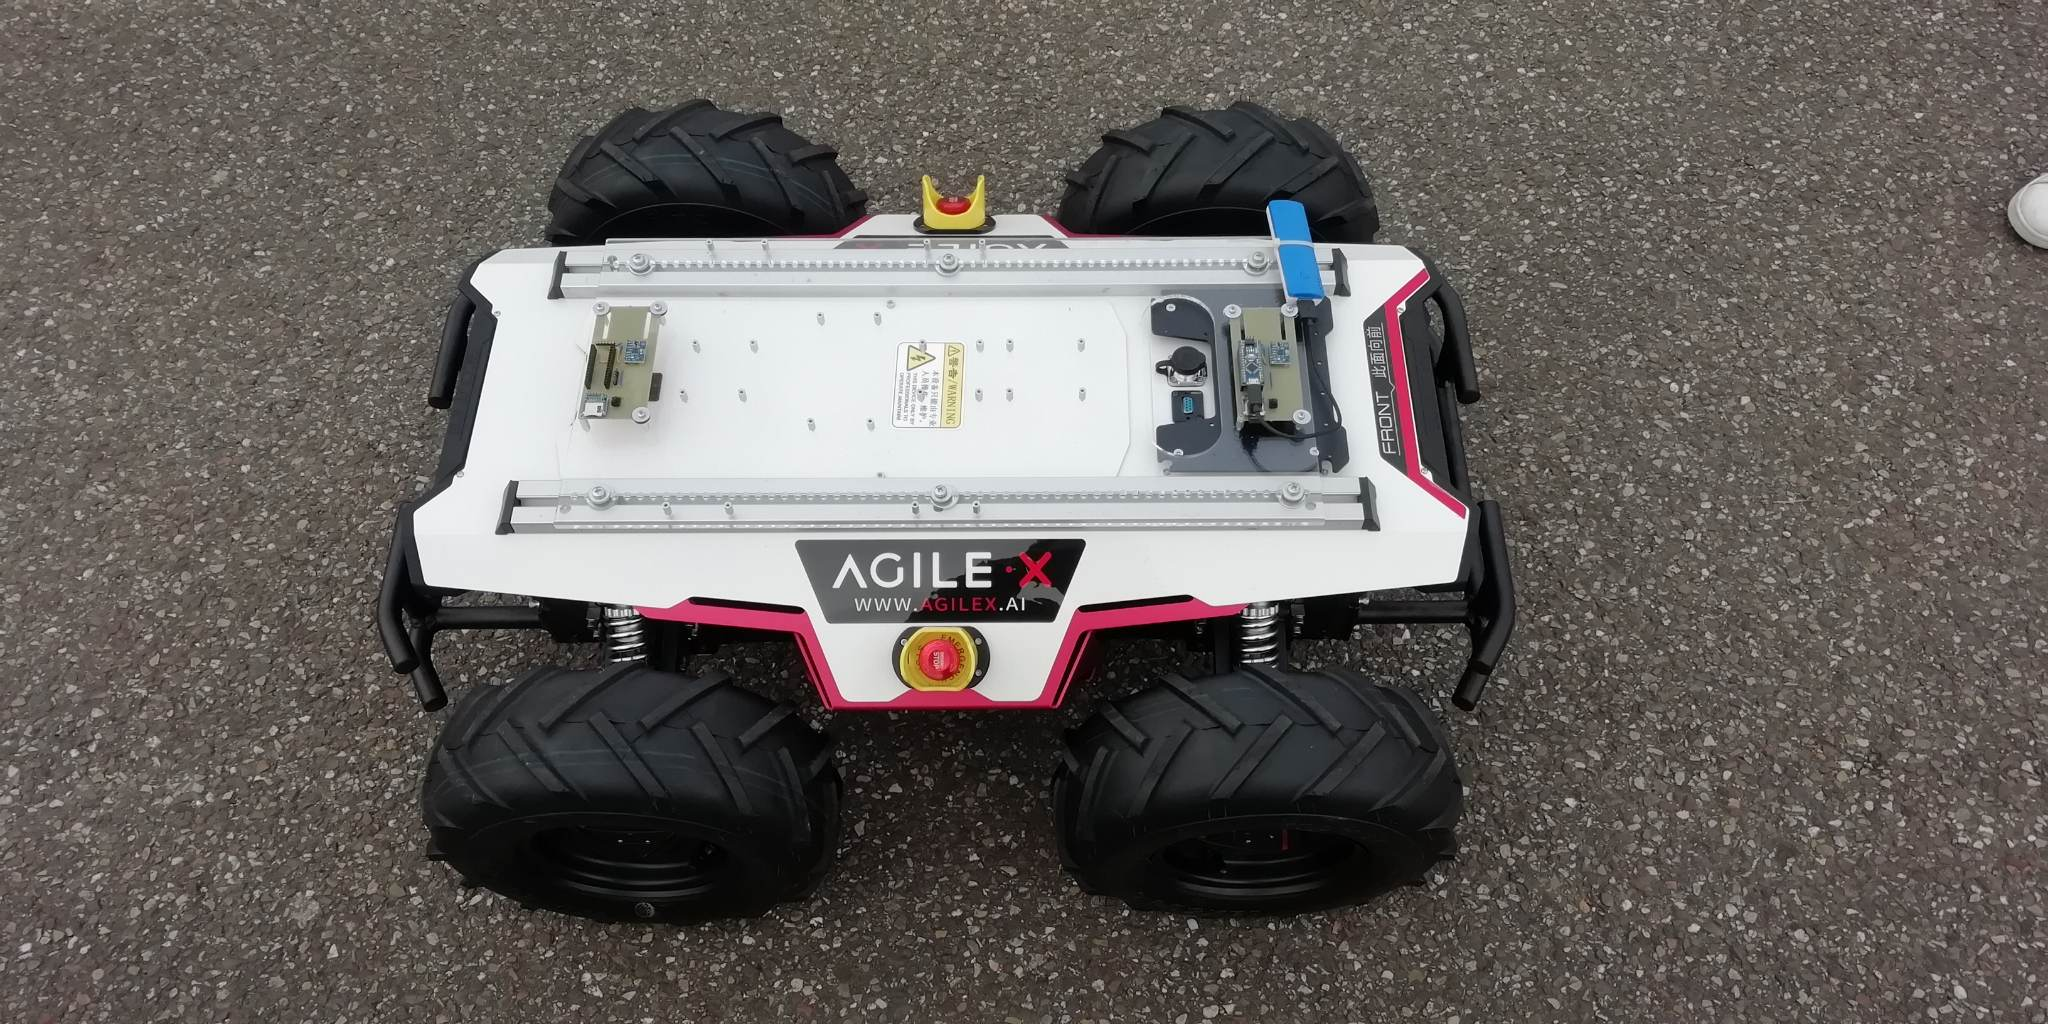
\includegraphics[scale=.15]{img/robot_1.png}
    \caption{First assembly of the Arduino devices on the robot vehicle}
    \label{robot_1}
\end{figure}

As using the robot takes a lot of time and effort, we prepared a detailed protocol beforehand describing all manipulations and data or metadata to collect. We also proposed some safety measures because the robot is both big, heavy and rather quick.\\

Unfortunately, the first use of the teleguided vehicle did not go as planned.\\
We had planned to use two Arduino devices by powering them with smartphones power banks because the robot was not yet ready to deliver 5v to the Arduino. Before any measurement, we noticed one of the battery was broken, leaving us with a unique recording device. Then, after a couple rides we tried to unload data from the micro SD card but there was none. Because the Arduino consumes so little power, the power bank was not detecting any charge and turned itself off... It was decided to use an old laptop straped with two wide elastics in order to provide power (Figure \ref{robot_2}) allowing us to reuse our second IMU. But either due to some damage inflicted to the recording device during a driving test or due to some micro SD card incompatibility (formatting format or too large capacity), the second Arduino device actually never recorded any data.

\begin{figure}
    \center
    \includegraphics[scale=.15]{img/robot_2.png}
    \caption{Final assembly of the Arduino devices on the robot vehicle}
    \label{robot_2}
\end{figure}

\subsection{Car}
The data collected from inside a car is quite different from our measurements on the robot.\\

First of all, the captor used to acquire accelerometric data is a smartphone accelerometer (utilised with an Android application named Physics Toolbox Sensor Suite). According to the person who performed the measurements, it was put on the passenger seat in the longitudinal direction for the first two recordings and sideways to the car for the last four collections.\\

Moreover there is GPS data associated with every recording. The position was not recorded by the smartphone but by a smartwatch.\\

In theroy, this new way of collecting data brings diversity to our dataset both in terms of vehicle and regarding degradations. The differents tracks contains new obstacles we cannot yet study with the robot such as: big speed-bumps, subsidences, manholes, bridge joints, rough strips, pavers and damaged pavement. But it remains to be seen if we can easily labelise the data using the driver's knowledge of the road.\\

\noindent
\begin{minipage}[!hc]{0.12\textwidth}
   \textbf{Remark}
\end{minipage}
\vrule\enskip\vrule\quad\begin{minipage}{\dimexpr 0.87\textwidth-0.8pt-1.5em}
As the mobile orientation is neither the same as the car's nor the same as real world coordinate system, a small program must be implemented in order to reproject acceleration data along relevant axis.
\end{minipage}

\subsection{Online Dataset}
A machine learning model needs an important amount of data to be trained. Collecting data ourselves is very laborious and labelising it would be very time consuming. So using online datasets would allow us to work with a larger and more diverse database.\\
A dataset containing a large amount of files was found online. These files mainly contains acceleration along the X, Y and Z axis of an unknown vehicle driving on top of some sort of obstacle (\textit{Metal bumps}) at two different speeds (unknown unit). Although these files looks to be suitable for AI training (labels and training/testing sets) it cannot be used unless we find more information about the data in contains.

% Data base ?